\chapter{Le robot logique}

	\marginicon{objectif}
	Dans ce chapitre nous allons appréhender les bases de la logique de
	programmation au travers d'une petite application
	ludique~: le «~robot logique~». Nous pourrons ainsi faire connaissance
	avec les concepts suivants~:
	
	\begin{liste}
	\item La séquence
	\item Les choix ou alternatives
	\item Les répétitions
	\item Les modules
	\end{liste}

	Il ne s'agit que d'une introduction;
	les chapitres suivants nous permettront d'approfondir
	ces concepts.

\section{Le «~robot logique~»}

	Pour introduire les bases de la logique de programmation, nous utilisons
	le «~robot logique~», un programme d'aide à
	l'apprentissage de l'algorithmique conçu par Marc Tommasi
	de l'université de Lille
	3\footnote{http://jrobot.gforge.inria.fr/}.
	
	\begin{center}
	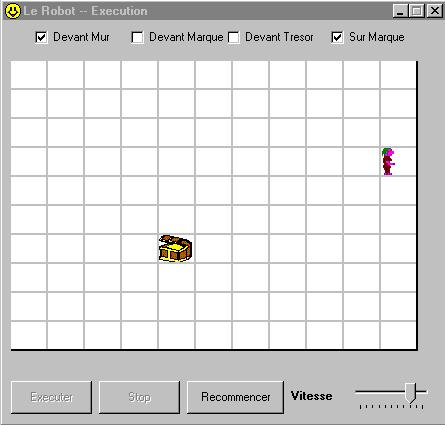
\includegraphics[width=5.553cm,height=5.302cm]{image/robot-grille}
	\end{center}
	
	Un robot se déplace dans un domaine rectangulaire sous 
	forme d'une grille délimitée par un mur.
	On peut y placer un trésor. Le but est de trouver
	l'algorithme qui va permettre au robot
	d'effectuer une tâche donnée (par exemple trouver le
	trésor). Pour cela, il faut combiner les ordres de base (les
	primitives) qu'il connait (par exemple~: «~avancer~»,
	«~à droite~», ...) en utilisant éventuellement des structures
	conditionnelles ou répétitives.

	\subsection{Installation}

		Le programme est pré-installé sur les machines de
		l'école mais il vous faudra
		l'installer chez vous. Nous vous indiquons comment
		installer la \textbf{version windows non maintenue}. Elle est plus
		simple à installer et à utiliser tout en étant suffisante pour ce que
		nous voulons en faire. Toutefois, elle ne fonctionne pas sous Linux ni
		sous Mac. Si vous êtes un utilisateur de ces systèmes, essayez
		d'installer la dernière version. Enfin, sachez que
		vous devez disposer des droits d'administration sur la
		machine pour l'installation.

		\marginicon{install}
		\begin{enumerate}
		\item
			Téléchargez le programme
			(\url{https://gforge.inria.fr/frs/?group\_id=2929})
		\item 
			Décompressez-le (avec le logiciel disponible sur votre machine)
		\item
			Cela crée un dossier «~robot~» avec un fichier \textit{Setup}.
			Exécutez-le.
		\end{enumerate}

	\subsection{Utilisation}

		Le robot se configure via deux fenêtres.

		\begin{enumerate}
		\item 
			La première permet d'indiquer la \textbf{situation
			initiale}~: position et orientation du robot, position du trésor.
		\item 
			La deuxième permet de «~programmer~» le robot, lui donner la
			\textbf{séquence d'instructions}
			qu'il va devoir suivre. Les instructions
			qu'il comprend sont rudimentaires. 
		\end{enumerate}

		Une troisième fenêtre montre la grille avec le robot et permet de voir
		«~tourner~» le programme.

\section{La séquence}

	Nous l'avons vu dans le chapitre
	d'introduction~: un algorithme est une séquence
	d'instructions élémentaires. Quelles sont les
	instructions élémentaires comprises par le robot ? Les instructions les
	plus rudimentaires sont~:
	
	\begin{Emphase}[definition]{Instructions élémentaires}
		\cadre{
		\begin{pseudo}
		\Stmt \K{Avancer}
		\Stmt \Comment Le robot se déplace d'une case dans la direction vers laquelle il regarde
		\Stmt \K{ADroite}
		\Stmt \Comment Le robot tourne d'un quart de tour vers la droite.
		\Stmt \Comment Ainsi, s'il regardait en bas, il regarde à présent à gauche.
		\end{pseudo}
		}
	\end{Emphase}
		
	Nous allons commencer par quelque chose de très simple~: demandons au
	robot de faire un demi-tour (sur place).

	\begin{Emphase}[exercice]{Exemple~: demi-tour}

		«~Faire demi-tour~» n'est pas une instruction
		élémentaire comprise par le robot. Il nous faut la découper en une
		séquence d'instructions plus simples. Ici, rien de
		compliqué, il suffit de tourner deux fois d'un quart
		de tour.

		\textbf{Conditions initiales}

		\begin{itemize}
		\item La position et la direction du robot sont aléatoires
		\item La position du trésor n'est pas importante
		\end{itemize}

		\textbf{But}~: Le robot doit faire demi-tour.

		\textbf{Solution}

		\cadre{
		\begin{pseudo}
		\Begin
			\Stmt ADroite
			\Stmt ADroite
		\End
		\end{pseudo}
		}
		
	\end{Emphase}

	Tentons à présent un exercice un peu plus compliqué
	(même si cela n'apparait pas tout de suite)

	
	\begin{Emphase}[exercice]{Exercice~: avancer de deux cases}

		\textbf{Conditions initiales}

		\begin{itemize}
		\item La position et la direction du robot sont aléatoires
		\item La position du trésor n'est pas importante
		\end{itemize}
		
		\textbf{But}~: Le robot doit avancer de deux cases dans la direction
		vers laquelle il regarde.

	\end{Emphase}

	Vous avez peut-être trouvé la solution suivante~:

	\cadre{
	\begin{pseudo}
	\Begin
		\Stmt Avancer
		\Stmt Avancer
	\End
	\end{pseudo}
	}
	
	Elle n'est \textbf{pas correcte} ! Pourtant je suis sûr
	que vous l'avez essayé et que le robot a effectivement
	avancé de 2 cases. 

	
	\begin{Emphase}[reflexion]{Test de l'algorithme}

		Si vous avez trouvé la solution ci-dessus, exécutez-la de nombreuses
		fois, vous finirez par tomber sur un cas où cela ne se passe pas bien.
		Pouvez-vous identifier quel est le problème ?

	\end{Emphase}

	Vous l'avez compris, si le robot est à moins de 2 cases
	du mur, il «~fonce~» dans le mur. Il signale ainsi
	qu'il ne peut pas exécuter une instruction du
	programme.
	
	\marginicon{attention}
	Ce n'est pas parce qu'un programme
	fonctionne correctement une fois, qu'il va fonctionner
	toujours. Il peut se produire un bug dans une condition qui
	n'a pas été prévue par le programmeur. Vous en avez
	sûrement tous déjà fait l'expérience avec les
	programmes que vous utilisez.

	Remarquez que le robot ne prend \textbf{jamais
	d'initiative}. Il exécute chaque instruction donnée
	sans se poser de question (est-ce pertinent, nécessaire ?). Il
	n'a d'ailleurs \textbf{aucune idée du
	but à atteindre, du sens de ce qu'il fait}.
	
	Ici, le problème vient également de
	l'énoncé qui ne stipule pas clairement ce
	qu'il faut faire dans ces cas-là.

\section{Poser correctement le problème}

	On a vu que notre robot «~fonce dans le mur~» si on lui demande
	d'avancer alors qu'il fait face à un
	mur. Il ne fait là qu'exécuter scrupuleusement
	l'algorithme qui lui a été fourni. Mais
	qu'aurait-il dû faire ? Nous n'en
	savons rien car l'énoncé ne le dit pas. On pourrait
	envisager que le robot s'arrête, fasse demi-tour,
	tourne en rond,\dots
	
	Cela met en évidence l'importance de la \textbf{phase
	d'analyse} dans le développement d'un
	programme. \textbf{Que faut-il faire exactement ?} Normalement la
	réponse est à chercher chez la personne pour qui on programme\footnote{Et
	à l'école, dans l'énoncé fourni par
	le professeur ! }.
	
	\marginicon{attention}
	Attention ! Ne surtout pas prendre d'initiative
	lorsqu'on programme. Si on ne sait pas quoi faire dans
	un cas précis, il faut repasser par la phase d'analyse
	pour le préciser. Sinon, on obtiendra la plupart du temps un programme
	\textbf{faux, car ne faisant pas ce qui est attendu}.

\section{Les alternatives}

	Reposons le problème précisément~: on veut que le robot avance de 2
	cases sauf si un mur l'en empêche, auquel cas il
	s'arrête juste devant le mur.
	
	À présent, la séquence d'instructions que le robot doit
	effectuer va dépendre de la situation, de son environnement. Comment
	faire ? Le robot a la possibilité de \textbf{tester son environnement}
	et de réagir en conséquence (en suivant scrupuleusement ce
	qu'on lui a \ indiqué évidemment). On va pouvoir lui
	donner deux séries d'instructions; il exécutera la
	première série ou la deuxième en fonction du résultat du test.

	
	\begin{Emphase}[definition]{Les tests}
	Les tests disponibles sont~:
	
		\cadre{
		\begin{pseudo}
		\Stmt \K{devantMur}
		\Stmt \Comment est vrai si le robot fait \textbf{face} à un mur.
		\Stmt \K{devantTrésor}
		\Stmt \Comment est vrai si le robot fait face au trésor.
		\Stmt \K{devantMarque}
		\Stmt \Comment est vrai si le robot fait face à une marque.
		\Stmt \K{surMarque}
		\Stmt \Comment est vrai si le robot est sur une marque.
		\Stmt \K{non}, \K{et}, \K{ou}
		\Stmt \Comment De plus, le robot est capable d'effectuer 
			des \emph{calculs logiques}
		\Stmt \Comment grâce à ces opérateurs.
		\end{pseudo}
		}
	\end{Emphase}

	
	\begin{Emphase}[definition]{Les alternatives}
		\cadre{
		\begin{pseudo}
		\If{condition}
			\Stmt série d'instructions à exécuter si la condition est vraie.
		\Else
			\Stmt série d'instructions à exécuter si la condition est fausse.
		\EndIf
		\end{pseudo}
		}
	\end{Emphase}

	Lorsque le robot doit exécuter une alternative, il teste la condition
	fournie. Si elle est vraie il exécute la première série
	d'instructions; sinon, il exécutera la seconde série.
	Ensuite, il passera à la suite de l'algorithme.

	On rencontrera souvent des situations ou la partie «~sinon~» est vide.
	Le robot doit effectuer des actions uniquement si la condition est
	vraie. Si elle est fausse, il ne doit rien faire (il passe à la suite
	du programme)

	\marginicon{attention}
	Une alternative est une instruction qui se place à un endroit précis
	dans la séquence d'instructions. Le robot ne
	l'évalue qu'à ce moment-là et agit en
	conséquence. Il ne s'agit absolument \textbf{pas de
	vérités} qu'on apprend à
	l'ordinateur, qui sont valables à tout moment et
	qu'il doit utiliser à bon escient pour améliorer son
	comportement.

	Ainsi on ne dit pas~: «~si, à un moment donné, tu es face à un mur,
	n'avance pas si on te le demande~» mais bien quelque
	chose comme~: «~si tu n'es pas devant un mur
	\textbf{MAINTENANT} alors tu peux avancer~»

	Notez aussi que le robot exécute \textbf{toutes} les instructions liées
	à un test même si cela en modifie le résultat. Ex: si on lui demande
	d'avancer deux fois s'il
	n'est pas devant le mur, il le fera même
	s'il se trouve devant le mur après le premier
	avancement.

	Comment utiliser les alternatives pour améliorer notre programme ?
	Commençons par un exemple simple.

	
	\begin{Emphase}[exercice]{Exemple~: avancer d'une case}

		\textbf{Conditions initiales}

		\begin{itemize}
		\item La position et la direction du robot sont aléatoires
		\item La position du trésor n'est pas importante
		\end{itemize}
		
		\textbf{But}~: Le robot doit avancer d'\textbf{une
		case} tout droit (dans la direction vers laquelle il regarde). 
		Si un mur l'en empêche, il devra s'arrêter juste devant ce mur.

	\end{Emphase}

	\cadre{
	\begin{pseudo}
	\Begin
		\If{non devantMur}
			\Stmt Avancer
		\Else
		\EndIf
	\End
	\end{pseudo}
	}
	
	Si cet exemple est bien compris, 
	essayez de résoudre par vous-même celui-ci~:

	
	\begin{Emphase}[exercice]{Exercice~: avancer de deux cases (amélioré)}

		\textbf{Conditions initiales}

		\begin{itemize}
		\item La position et la direction du robot sont aléatoires
		\item La position du trésor n'est pas importante
		\end{itemize}
		
		\textbf{But}~: Le robot doit avancer de \textbf{deux cases} tout droit
		(dans la direction vers laquelle il regarde). Si un mur
		l'en empêche, il devra s'arrêter
		juste devant le mur.

	\end{Emphase}

\section{La répétition}

	Continuons notre apprentissage de l'algorithmique et
	posons-nous le problème suivant~: «~On voudrait que le robot avance
	\textbf{jusqu'au} mur face à lui.~».
	
	Que se passe-t-il ici ? Le robot va devoir avancer un certain nombre de
	fois mais ce nombre est inconnu au moment de
	l'écriture de l'algorithme; cela va
	dépendre de la situation initiale. Nous allons nous en sortir grâce à
	la structure répétitive. On peut demander à
	l'ordinateur de \textbf{répéter} des instructions. On
	lui fournit également une condition qui lui permet de savoir
	s'il doit continuer ou non cette tâche répétitive.

	
	\begin{Emphase}[definition]{La répétition}
	\cadre{
	\begin{pseudo}
		\While{condition}
			\Stmt série d'instructions à exécuter si la condition est vraie.
		\EndWhile
	\end{pseudo}
	}
	\end{Emphase}

	Lorsqu'il rencontre cette structure, le robot évalue la
	condition. Si elle est vraie, il exécute \textbf{toutes} les
	instructions à l'intérieur du «~\textit{tant que~}»
	puis revient tester la condition. Lorsqu'elle devient
	fausse ou si elle est fausse dès le début, il passe à la suite de
	l'algorithme.
	
	Nous avons à présent tout ce qu'il faut pour résoudre
	notre problème.

	
	\begin{Emphase}[exercice]{Exercice~: avancer jusqu'au mur}

		\textbf{Conditions initiales}

		\begin{itemize}
		\item La position et la direction du robot sont aléatoires
		\item La position du trésor n'est pas importante
		\end{itemize}
		
		\textbf{But}~: Le robot doit avancer jusqu'au mur
		devant lui et s'y arrêter.

	\end{Emphase}

\section{Les marques du robot}

	Imaginons à présent que l'on veuille que le robot
	revienne à sa position de départ après avoir atteint le mur. Le
	problème c'est que le robot n'a pas
	de mémoire. Par contre, il peut laisser une trace de son passage
	(tracer une croix sur la case qu'il occupe).
	
	\marginicon{attention}
	Un ordinateur, lui, possède une mémoire. Il pourrait ainsi retenir les
	coordonnées de la case de départ ou encore le nombre de cases
	parcourues avant d'arriver au mur.

	
	\begin{Emphase}[definition]{Instructions élémentaires}
		\cadre{
		\begin{pseudo}
		\Stmt \K{ajouterMarque} 
		\Stmt \Comment Le robot trace une croix sur la case qu'il occupe.
		\Stmt \K{effacerMarque}
		\Stmt \Comment Le robot efface la croix sur la case qu'il occupe.
		\end{pseudo}
		}
	\end{Emphase}

	\begin{Emphase}{Test}
		\cadre{
		\begin{pseudo}
		\Stmt \K{surMarque}
		\Stmt \Comment Est vrai si le robot est dans une case marquée d'une croix.
		\end{pseudo}
		}
	\end{Emphase}

	Nous avons à présent tout ce qu'il faut pour résoudre
	notre problème. Il est déjà d'une belle complexité
	mais vous avez tout ce qu'il faut pour le résoudre~:
	courage !

	
	\begin{Emphase}[exercice]{Exercice~: avancer jusqu'au mur et revenir}

		\textbf{Conditions initiales}

		\begin{itemize}
		\item La position et la direction du robot sont aléatoires
		\item La position du trésor n'est pas importante
		\end{itemize}
		
		\textbf{But}~: Le robot doit avancer jusqu'au mur
		devant lui, faire demi-tour et revenir à sa position de départ.

	\end{Emphase}

\section{La notion de procédure}

	Pour le problème précédent, vous avez dû, par deux fois, demander au
	robot de faire demi-tour. C'est un problème que vous
	aviez déjà résolu au début de ce chapitre mais vous avez dû, à nouveau,
	expliquer au robot comment faire. C'est gênant !

	\begin{liste}
	\item 
		L'algorithme devient répétitif car il contient du code dupliqué
		(deux fois «~à droite~»).
	\item 
		À la lecture de l'algorithme, 
		il n'apparait pas clairement qu'on demande au robot 
		d'effectuer un demi-tour
		(en tout cas moins clairement que si on trouvait explicitement
		l'ordre «~demi-tour~»).
	\end{liste}

	\marginicon{reflexion}
	Pourquoi est-ce important que l'algorithme soit lisible
	par un humain puisque c'est le robot
	(l'ordinateur si on généralise) qui va le lire et
	l'exécuter ?

	La solution au problème de duplication de code est fournie par la notion
	de \textit{procédure}.

	\marginicon{definition}
	Une \textbf{procédure} (on dira aussi \textbf{module}, \textbf{fonction}
	ou \textbf{méthode}) est une portion d'algorithme
	auquel on a donné un \textbf{nom} et qui peut être «~utilisé~»
	(\textbf{appelé}) dans d'autres algorithmes.

	Lorsque le robot rencontre un nom de procédure, il exécute toutes les
	instructions de cette procédure puis revient continuer le premier
	algorithme là où il a été interrompu.

	Exemple~: L'algorithme A appelle la procédure «~Brol~».

	\begin{center}
	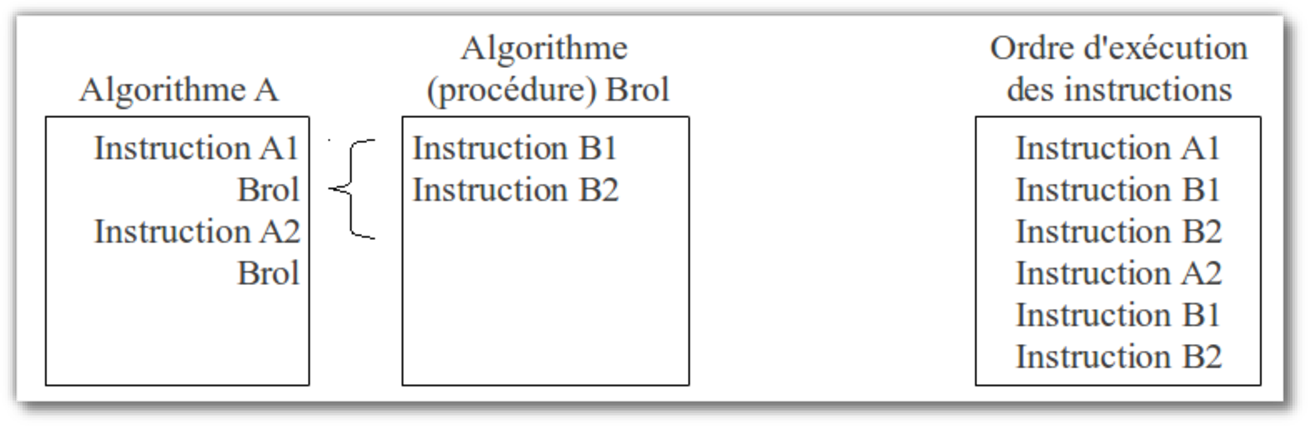
\includegraphics[width=\textwidth]{image/robot-procedure}
	
	{Remarque~: une procédure est également un algorithme !}
	\end{center}

	
	\begin{Emphase}[exercice]{Exercice~: procédure pour le demi-tour}
	
		Écrire une procédure «~demi-tour~» et l'utiliser dans
		le problème précédent (avancer jusqu'au mur et revenir
		au point de départ).
		
		Que pourrions-nous encore écrire comme procédure pour accroitre
		la lisibilité de notre algorithme ?

	\end{Emphase}

\section{Conclusion}

	Le robot nous a permis d'appréhender les principaux
	concepts de l'algorithmique qui vont maintenant nous
	servir pour programmer un ordinateur. 
	
	Une différence importante entre le robot et
	l'ordinateur est que ce dernier possède une
	«~mémoire~» que nous allons pouvoir exploiter au travers du concept de
	variable.

\section{Exercices}

	\subsection{Exercices de réflexion}

		\textit{
		Pour ces exercices, on vous demande de réfléchir sur le concept
		d'algorithme.}

\begin{Exercice}{Un algorithme correct}
Quand peut-on affirmer qu'un algorithme est correct ?
\end{Exercice}

\begin{Exercice}{Unicité d'un algorithme}
	Est-il, selon vous, possible de trouver 
	plusieurs algorithmes différents
	pour résoudre un même problème ?
\end{Exercice}

\begin{Exercice}{Un problème insoluble}
	Pouvez-vous imaginer un problème insoluble pour le robot ?
	C'est-à-dire un problème pour lequel on ne peut pas
	trouver d'algorithme qui le résolve.
\end{Exercice}

	\subsection{Séquences simples}
	
		Pour les exercices suivants, le robot se trouve 
		au départ dans le coin sud-ouest, 
		orienté vers le nord.

\begin{Exercice}{Avancer simplement}
	Le robot doit avancer de trois cases.
\end{Exercice}

\begin{Exercice}{Avancer et tourner}
	Le robot doit avancer de trois cases, tourner à droite, 
	avancer de cinq cases.
\end{Exercice}

\begin{Exercice}{Aller-retour}
	Le robot doit avancer de trois cases, demi-tour, 
	revenir au départ, demi-tour.
\end{Exercice}

\begin{Exercice}{Le carré}
	Le robot se promène sur la grille 
	et décrit un carré de quatre cases sur quatre.
\end{Exercice}
		
	\subsection{Alternatives}

\begin{Exercice}{Avancer d'une case}
	Le robot est placé au hasard.
	Le robot avance si la case devant lui est libre (pas devant un mur).
\end{Exercice}

\begin{Exercice}{Avancer ou demi-tour}
	Le robot est placé au hasard. 
	Le robot avance si la case devant lui est libre,
	sinon il fait demi-tour.
\end{Exercice}

\begin{Exercice}{Chercher le trésor devant}
	Le robot se trouve dans le coin nord-est, orienté vers
	l'ouest; le trésor est au nord. Le robot doit avancer
	de deux cases au plus. Si le robot se trouve devant le trésor lors de
	son déplacement, il est si content qu'il fait un tour
	sur place avant de se jeter dessus.
\end{Exercice}

\begin{Exercice}{Avancer de deux cases}
	Le robot est placé au hasard. Il avance de 2 cases.
\end{Exercice}


	\subsection{Répétitives}

		\emph{%
		À partir d'ici, les exercices sont difficiles
		(en tout cas en début d'année; en fin d'année,
		ils devraient vous paraitre plus faciles).
		Si vous n'y arrivez pas tout de suite, c'est normal; 
		vous pourrez y revenir de temps en temps 
		tout au long de votre apprentissage.
		}

		Le robot se trouve dans le coin sud-ouest, orienté vers le nord.

		\begin{Exercice}{Nord-ouest}
			Le robot doit aller jusqu'au coin nord-ouest.
		\end{Exercice}

		\begin{Exercice}{Nord-ouest et retour}
			Le robot doit aller jusqu'au coin nord-ouest
			puis revenir sur sa case de départ par le même chemin.
		\end{Exercice}

		\begin{Exercice}{Nord-est}
			Le robot doit aller jusqu'au coin nord-est.
		\end{Exercice}

		\begin{Exercice}{Trésor}
			Le robot doit aller jusqu'au trésor qui se trouve
			\begin{itemize}
			\item soit dans le coin nord-est ;
			\item soit dans le coin nord-ouest.
			\end{itemize}
		\end{Exercice}

	\subsection{Modules}

		\begin{Exercice}{Demi-tour}
			Écrire un module qui fait faire un demi-tour au robot.
		\end{Exercice}

		\begin{Exercice}{Tourner}
			Écrire un module qui fait tourner le robot à gauche.
		\end{Exercice}

		\begin{Exercice}{Mur}
			Écrire un module qui déplace le robot
			jusqu'au mur devant lui.
		\end{Exercice}

		\begin{Exercice}{Mur ou trésor}
			Écrire un module qui déplace le robot jusqu'au mur
			devant lui ou le trésor s'il est sur le chemin.
		\end{Exercice}

		\begin{Exercice}{Coin nord-ouest}
			Écrire un module qui déplace le robot vers le coin nord-ouest 
			(orienté vers l'est); on suppose qu'au départ
			le robot est orienté vers l'est.
		\end{Exercice}

		\begin{Exercice}{Un coin}
			Le robot est placé au hasard. 
			Écrire un module qui va dans un coin, peu
			importe lequel. 
		\end{Exercice}

	\subsection{Challenge}

		\begin{Exercice}{Tour du domaine}
			Le robot doit faire le tour du domaine en marquant toutes les cases du
			pourtour, et revenir ensuite à sa position (et son orientation) de
			départ.

			\begin{itemize}
			\item Le robot est situé dans le coin supérieur gauche et regarde à droite.
			\item La position du trésor n'est pas importante.
			\end{itemize}

			\textbf{Conseil}~: L'utilisation de procédures rendra
			votre programme plus court et plus lisible.
		\end{Exercice}

		\begin{Exercice}{Trouver le trésor (1°)}
			Le robot doit s'arrêter sur le trésor.

			\begin{itemize}
			\item Le robot est situé dans le coin supérieur gauche et regarde à droite.
			\item Le trésor est sur le bord supérieur.
			\end{itemize}

			\textbf{Attention}~: 
			Testez bien votre solution; il existe un cas très particulier.
		\end{Exercice}

		\begin{Exercice}{Trouver le trésor (2°)}
			Le robot doit s'arrêter sur le trésor.

			\begin{itemize}
			\item Le robot est placé aléatoirement et regarde une direction à droite.
			\item Le trésor est placé sur le bord droit.
			\end{itemize}
		\end{Exercice}

		\begin{Exercice}{Trouver le trésor (3°)}
			Le robot doit s'arrêter sur le trésor.

			\begin{itemize}
			\item Le robot est placé aléatoirement et regarde une direction au hasard.
			\item Le trésor est placé sur un bord au hasard.
			\end{itemize}
		\end{Exercice}

		\begin{Exercice}{Marquer le domaine}
			Le robot doit marquer \textbf{complètement} le domaine
			(totalement vide au départ). 
			L'ordre dans lequel il trace les croix n'est pas important.

			\begin{itemize}
			\item
				À vous de choisir la situation initiale du robot qui vous permet de
				résoudre au mieux le problème.
			\end{itemize}
		\end{Exercice}

		\begin{Exercice}{Trouver le trésor (4°)}
			Le robot doit s'arrêter sur le trésor.

			\begin{itemize}
			\item Le robot est situé dans le coin supérieur gauche et regarde à droite.
			\item Le trésor est placé au hasard.
			\end{itemize}
		\end{Exercice}

		\begin{Exercice}{Trouver le trésor (5°)}
			Le robot doit s'arrêter sur le trésor.

			\begin{itemize}
			\item Le robot est placé aléatoirement et regarde une direction au hasard.
			\item Le trésor est placé au hasard.
			\end{itemize}
		\end{Exercice}
			
